
The constitutive model presented in section \ref{sec:constitutive equations} is general and can be applied to a wide variety of materials. In the context of EAPs, multiple authors have performed experimental testing, of the single physics, such as mechanical, thermal or electrical behavior (\cite{Hossain2012visco, Dippel2015}) as well as the coupled behavior of the combination of two (\cite{Liao_Mokarram2020, Alkhoury2022}) or the three physics (\cite{Mehnert2021a,Sheng2012, Qin2023}). The data reported in the literature will be used to calibrate a constitutive model for VHB polymer, where the calibration involves the choice of specific mechanical models and thermal functions, fitting the best parameters and estimating an error for the model.

Beyond finding optimal parameters, the scope of the calibration is to validate the theoretical formulation and to show its capabilities. The proposed framework is valid for other materials and the methodology shows some conclusions that can be applied for other material caracterization.


\subsection{Experiment protocols and data availability}

For the accurate calibration of VHB polymer, data from the literature has been collected and classified. The selected experimental tests can be classified in the following groups: differential scanning calorimetry (DSC), one-cycle loading-unloading tests, creep tests at constant deformation, quasi-static loading and broadband dielectric spectrometry (BDS). Mechanical as well as electrical tests provide data at different temperatures, covering a range from \si{-20\celsius} up to \si{80\celsius}. Some of the tests are very specific and allow to calibrate a single parameter of a very narrow set of parameters. Other tests like cyclic loading involve the copupling of the thermal, elastic and viscous effects.


\begin{figure}[htbp]
  \centering
  \begin{subfigure}{0.48\textwidth}
    
\includegraphics[width=\textwidth]{figures/qualitative_experim_calorimetry.pdf}
    \caption{DSC}
    \label{fig:selected_experim_dsc}
  \end{subfigure}
  \hfill
  \begin{subfigure}{0.48\textwidth}
    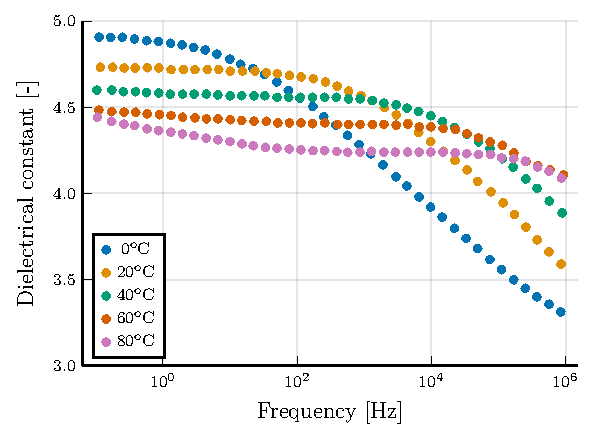
\includegraphics[width=\textwidth]{figures/qualitative_experim_dielectrical.pdf}
    \caption{BDS}
    \label{fig:selected_experim_bds}
  \end{subfigure}
  \vspace{1em}
  \begin{subfigure}{0.48\textwidth}
    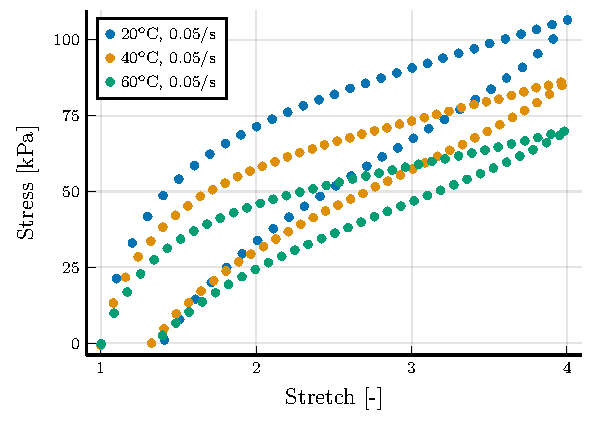
\includegraphics[width=\textwidth]{figures/qualitative_experim_one_cycle.pdf}
    \caption{Loading-unloading}
    \label{fig:selected_experim_load}
  \end{subfigure}
  \hfill
  \begin{subfigure}{0.48\textwidth}
    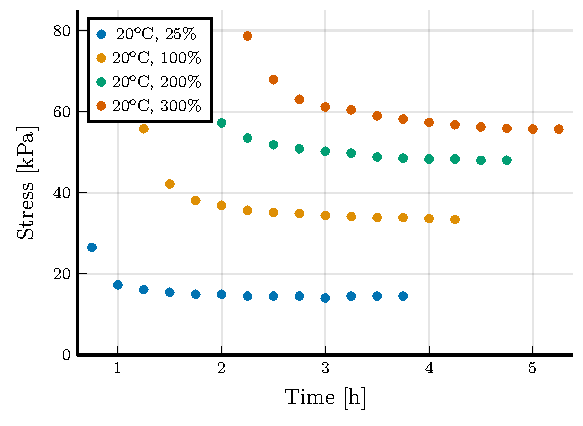
\includegraphics[width=\textwidth]{figures/qualitative_experim_creep.pdf}
    \caption{Creep}
    \label{fig:selected_experim_creep}
  \end{subfigure}
  \caption{Visualization of selected experiments showing the thermo-electro-mechanical response of the material.}
  \label{fig:selected_experiments}
\end{figure}


The most relevat experiments that will be used in the calibration of the consitutive model are shown in figure (\ref{fig:selected_experiments}). DSC and BDS experiments follow standarized protocols and more information can be found in \cite{Hohne2003_DSC} and \cite{Kremer2003_BDS} respectively. This two experiments allo to identify specific heat and dielectrical properties in the absence of mechanical actions.

Mechanical tests can be of different types, such as cyclic loading, quasi-static loading, and creep at constant stretch. Creep tests are a subtype of cyclic loading at a very low velocity and coincide with the assimptotic stress of the creep tests. These experiments are widely used for the mechanical characterization of viscoelastic materials, however, they are not standarized and the loading protocols can be vary accross laboratories and authors. Understanding the loading protocols is needed to define the numerical simulation of experiments and thus, to perform an optimization for the material parameters.


\begin{table}[htbp]
\centering
\caption{Types and sources of experimental data.}
\label{tab:experiment_sources}
\begin{tabular}{@{}llc@{}}
\toprule
Data Set & Experiment Type & Reference \\
\midrule
Set 1 & Differential scanning calorimetry (DSC)            & \cite{Dippel2015} \\
Set 2 & One-cycle loading-unloading                        & \cite{Liao_Mokarram2020} \\
Set 3 & Constant stretch creep                             & \cite{Liao_Mokarram2020} \\
Set 4 & Quasi-static loading                               & \cite{Liao_Mokarram2020} \\
Set 5 & One-cycle loading-unloading (discarded)            & \cite{Alkhoury2022} \\
Set 6 & Constant stretch creep (discarded)                 & \cite{Alkhoury2022} \\
Set 7 & Broadband dielectrical spectrography (BDS)         & \cite{Sheng2012} \\
Set 8 & Thermo-electro-mechanical one-cycle loading-unloading & \cite{Mehnert2021a} \\
\bottomrule
\end{tabular}
\end{table}


The mechanical tests reported in \cite{Liao_Mokarram2020,Alkhoury2022} describe the following 


Another important consideration is that the stresses reported by different authors under the same conditions of temeprature, velocity and stretch may be different. This observation would open a discussion about uncertainity of the material data and error propagation. Given the scope of this investigation is to assess the suitability of the numerical model to predict the behavior of EAPs, only consistent data will be considered. The differences on the experimental measurements could be of different sources: VHB polymer is manufactured as an adhesive tape, hence, quality control focus on properties different from viscoelastic behavior; VHB polymer is provided in different thicknesses, which can affect the curing process of the polymer; and finally, engineering tolerances are not defined for the analyzed properties and can very from one batch of production to another.


\subsection{Constitutive model calibration}


\subsection{Validation and error estimation}


\subsection{Conclusions}


